\chapter{Introduction}



Machine learning is a  field of computer science that concerned with data processing and the ability
of the computer to learn from this data. 
One main objective of this field is the development of algorithms capable of inference based on 
observable data, such as text documents, pictures, audio, video etc.. 
 
In the \textit{Supervised Learning} setting, the input of the learning algorithm are input-label pairs. 
The goal of the algorithm is to learn the underlying connection between the inputs and their labels, 
thus being able to \textit{predict} a label for a previously unseen input. 
When the possible label values are from a discrete finite set, this learning problem is called
 \textit{classification}. The basic classification problem is the \textit{binary classification}, i.e. classifying 
 each data instance into one of only two possible classes. In contradiction to 
 the , the classification task in the binary 
 case is more simple because, eliminating one class , gives you the correct one 
 straightforward. However, this is more difficult in the \textit{multiclass 
 classification}, when even when we eliminate one possible class, we still have 
 some more classes the we need to decide which is the correct one. 
 

\subsection{Online learning}

One of the main features of the classification problem is the way how the data is been collected. 
Assume you want to buy a house. There are two ways to do that. 
You can pay all the house cost at once and you get the house, or, 
if you don't have all the money right now but you do want to get into the house as soon as possible, 
 you can pay a mortgage every month and become closer and closer to a full ownership each month. 
 Collecting a data as  collecting money can be done in two ways. 
 In the \textit{Batch learning} setting we collect a certain amount of data first, and  than, 
 we want to use this data in order to learn how to classify the incoming data instances. 
 However, in a lot of applications there is a flow of data that is transmitted in sequence  
 and we would like to learn on the flow how to classify the data instances. 
 The last method is called \textit{Online Learning}.

Unlike the \textit{Batch learning}, in \textit{Online Learning} 
 the learner perception about the classification task become stronger when the time is pass by.

The \textit{Online Learning} is performed in rounds, where in each round $t$, 
the algorithm gets an input instance $\vxii$ in some domain $\mathcal{X}$  and predicts a  correspond 
measure, $\hat{p_t}$ based on the algorithm decision  rule. This measure can be in the label domain, 
$\mathcal{Y}$ , or can be mapped into $\hat{y_t}$ which is the predicted label in $\mathcal{Y}$ .   
After predicting the label , the true label, $y_t$ in the labels domain, $\mathcal{Y}$, is revealed 
and the learner suffers a non negative loss of $\l\paren{\hat{p_t},y_t}$ that measures how much the 
prediction is compatible with the true label. The desired property of such function is to generate low 
values when the prediction is close to the actual label in some sense, and high values when the opposite 
is true. Then, the algorithm update its decision rule based on the past known data and the revealed label. 

\subsection{Selective Sampling}

Usually, in an   online binary learning task setting,  we improve the prediction over the time, 
which means that the algorithm improves performance during the time and have less and lees prediction
 mistakes when it updates its model. 
Sometimes , annotating the data consume expensive resources, like time, money or manpower, 
and we would like to avoid using this resources when we can. In other words, we would like 
to avoid querying labels for the input examples when it is possible. For example, if we need to update the 
model only when there is a prediction mistake (as in Perceptron), we actually don't really 
use the information about the correct label when there is no need to update. In such cases, 
it will be helpful to assess every time if we sure about our prediction, and no update should be done, 
so no query should be issued, or if we not sure about the prediction, hence we should issue a 
query and update the model using the update rule an the correct label. 
This approach, that queries labels only for selected examples is called \textit{Selective sampling.}

This work deals with multi-task problem where $K$ learners are sharing a single annotator with limited bandwidth. This limitation allow only one task to get feedback from the annotator at a time. For example, there is a need to label annotate news items from few agencies, one person can not handle all of them, and some can just be annotated. Our setting is designed to handle exactly this problem, and specifically, how to make best usage of annotation time. 

\section{Prolem Setting}
\label{sec:setting}
We study online multi-task learning with a shared annotator. In our setting, there are
$K$  binary classification tasks to be learned simultaneously. 
No dependency between the tasks is assumed during the analysis, but the tasks can be dependent as well. 
Learning is performed in rounds as an online learning algorithm, as following: 
On each round $t$, there are $K$ input-label pairs
$(\vxi{i,t},\yi{i,t})$ where $i=1,2\comdots K$ is the task index and $t$ is the step index. The inputs $\vxi{i,t}\in\reals^{d_i}$ are
vectors, and labels  $\yi{i,t}\in\{-1,+1\}$ are binary. In the general
case, the input-spaces for each problem may be different, and inputs may
have different number of elements. Yet, in order to  simplify the notation and without loss of generality,  from now
on, for our analysis we assume that for all of the tasks, $\vxi{i,t}\in\reals^{d}$. i.e. all the tasks are in the same dimension and   $d_i = d$ holds for all tasks . 


On round $t$, the learning algorithm receives $K$ inputs $\vxi{i,t}$
for $i=1 \comdots K$ tasks and outputs $K$ binary-labels $\hyi{i,t}$, where
$\hyi{i,t}\in\{-1,+1\}$ is the label predicted for the input
$\vxi{i,t}$ of task $i$. The algorithm then chooses a task $J_t \in\
\{1 \comdots K\}$ and receives from an annotator its true-label
$\yi{J_t,t}$ for that task $J_t$. Unlike the usual online multi-task setting, it  does not observe any other
label. Then, the algorithm updates its models, using the received feedback, and proceeds to the
next round (and inputs).  For the ease of calculations below, we denote
by $K$ indicators $Z_t=\paren{ Z_{1,t} \comdots Z_{K,t}}$, the
identity of the task which was queried on round $t$, and set
$Z_{J_t,t}=1$ and $Z_{i,t}=0$ for $i\ne J_t$. Clearly from the definition, the condition, $\sum_i
Z_{i,t}=1 ,\forall{i,t}$, always holds . Below, we define the notation $\Expp{t-1}{x}$ to be the
conditional expectation $\Exp{x \vert Z_{1},...Z_{t-1}}$ given all
previous choices of the tasks to be queried.


Schematic illustration of a single iteration of multi-problem algorithms is shown in \figref{fig:ilustration}. The top panel shows the standard
setting of online multi-task algorithms with a shared annotator, that labels all inputs, which are fed to the corresponding algorithms to update corresponding models. The
bottom panel shows the SHAMPO algorithm, which couples labeling
annotation and learning process, and synchronizes a single annotation
per round.  At most one task performs an update per round, the one
with the annotated input.

\begin{figure}
\begin{centering}
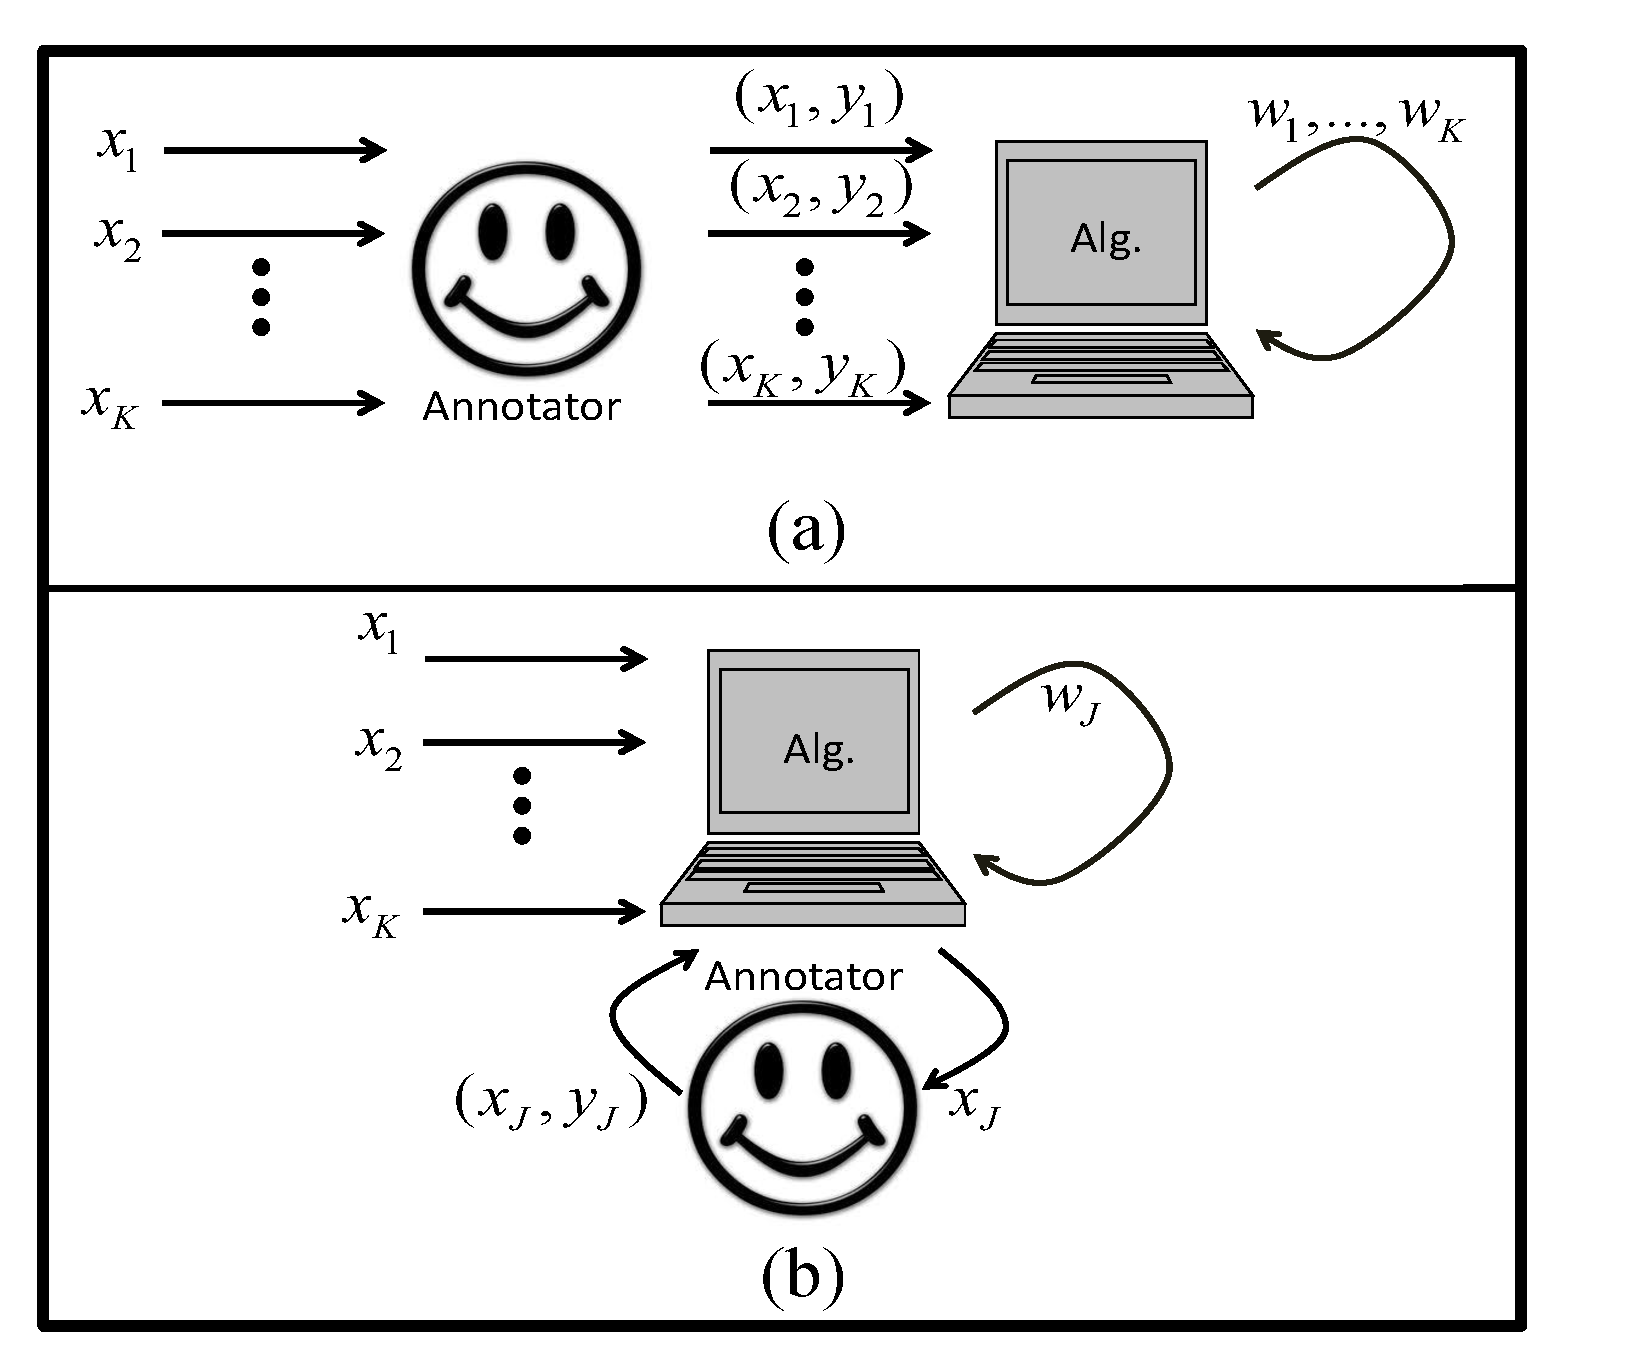
\includegraphics[width=0.5\textwidth]{figs/SHAMPO_illustration.eps}
\caption{Illustration of a single iteration of  multi-task algorithms (a) standard setting, shared annotator labels all inputs, and algorithms update models. (b) SHAMPO algorithm couples labeling annotation and learning process, and synchronizes a single annotation per round.}
\label{fig:ilustration}
\end{centering}
\end{figure}

\begin{figure}
\begin{centering}
\includegraphics[width=0.7\textwidth]{figs/table_ss.eps}
\end{centering} 
%\vspace{10}
\begin{centering}
\includegraphics[width=0.7\textwidth]{figs/table_SHAMPO.eps}
\caption{In selective sampling we focus on when to issue a query for a single task (a row), while in the SHAMPO setting we
   COMPLETE THIS SENTENCE  }
\label{fig:ss_vs_SHAMPO}
\end{centering}
\end{figure}

\fbox{to do - background in multi-armed bandits. and show the simple perceptron
}
